This Appendix contains the pull plots for the \wh{} SRs.

% \begin{figure}[htp]
%   \centering
%   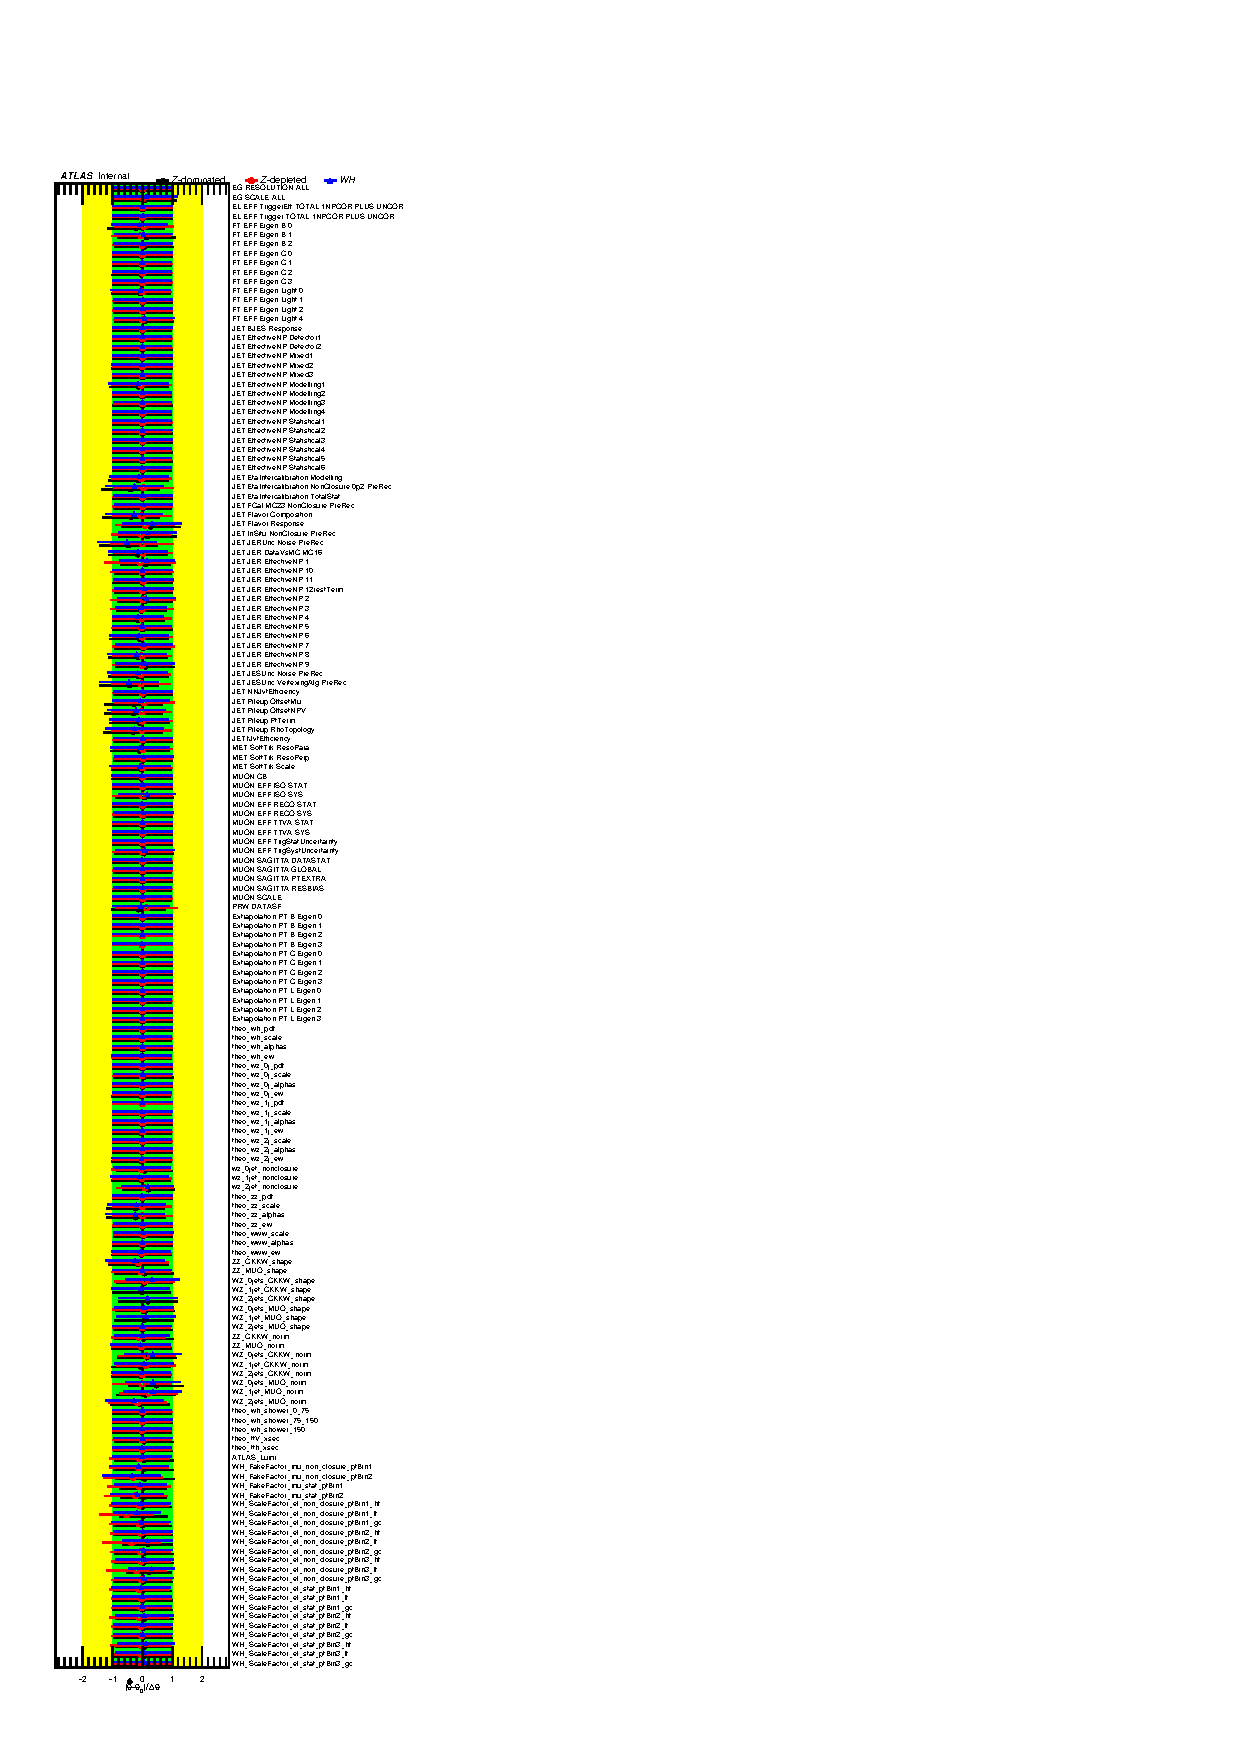
\includegraphics[width=0.33\linewidth]{figures/appendix/wh_results/pulls/NuisPar_comp.pdf}
%   \caption{Systematic uncertainty pull plot. The black lines represent the \zdom{} pulls, red lines the \zdep{} pulls, and the blue lines the combined fit.}\label{fig:wh_pull_plots_zdom_zdep_expected}
% \end{figure}

\begin{figure}[htp]
  \centering
  \subfloat[\zdom{} SR.]{
    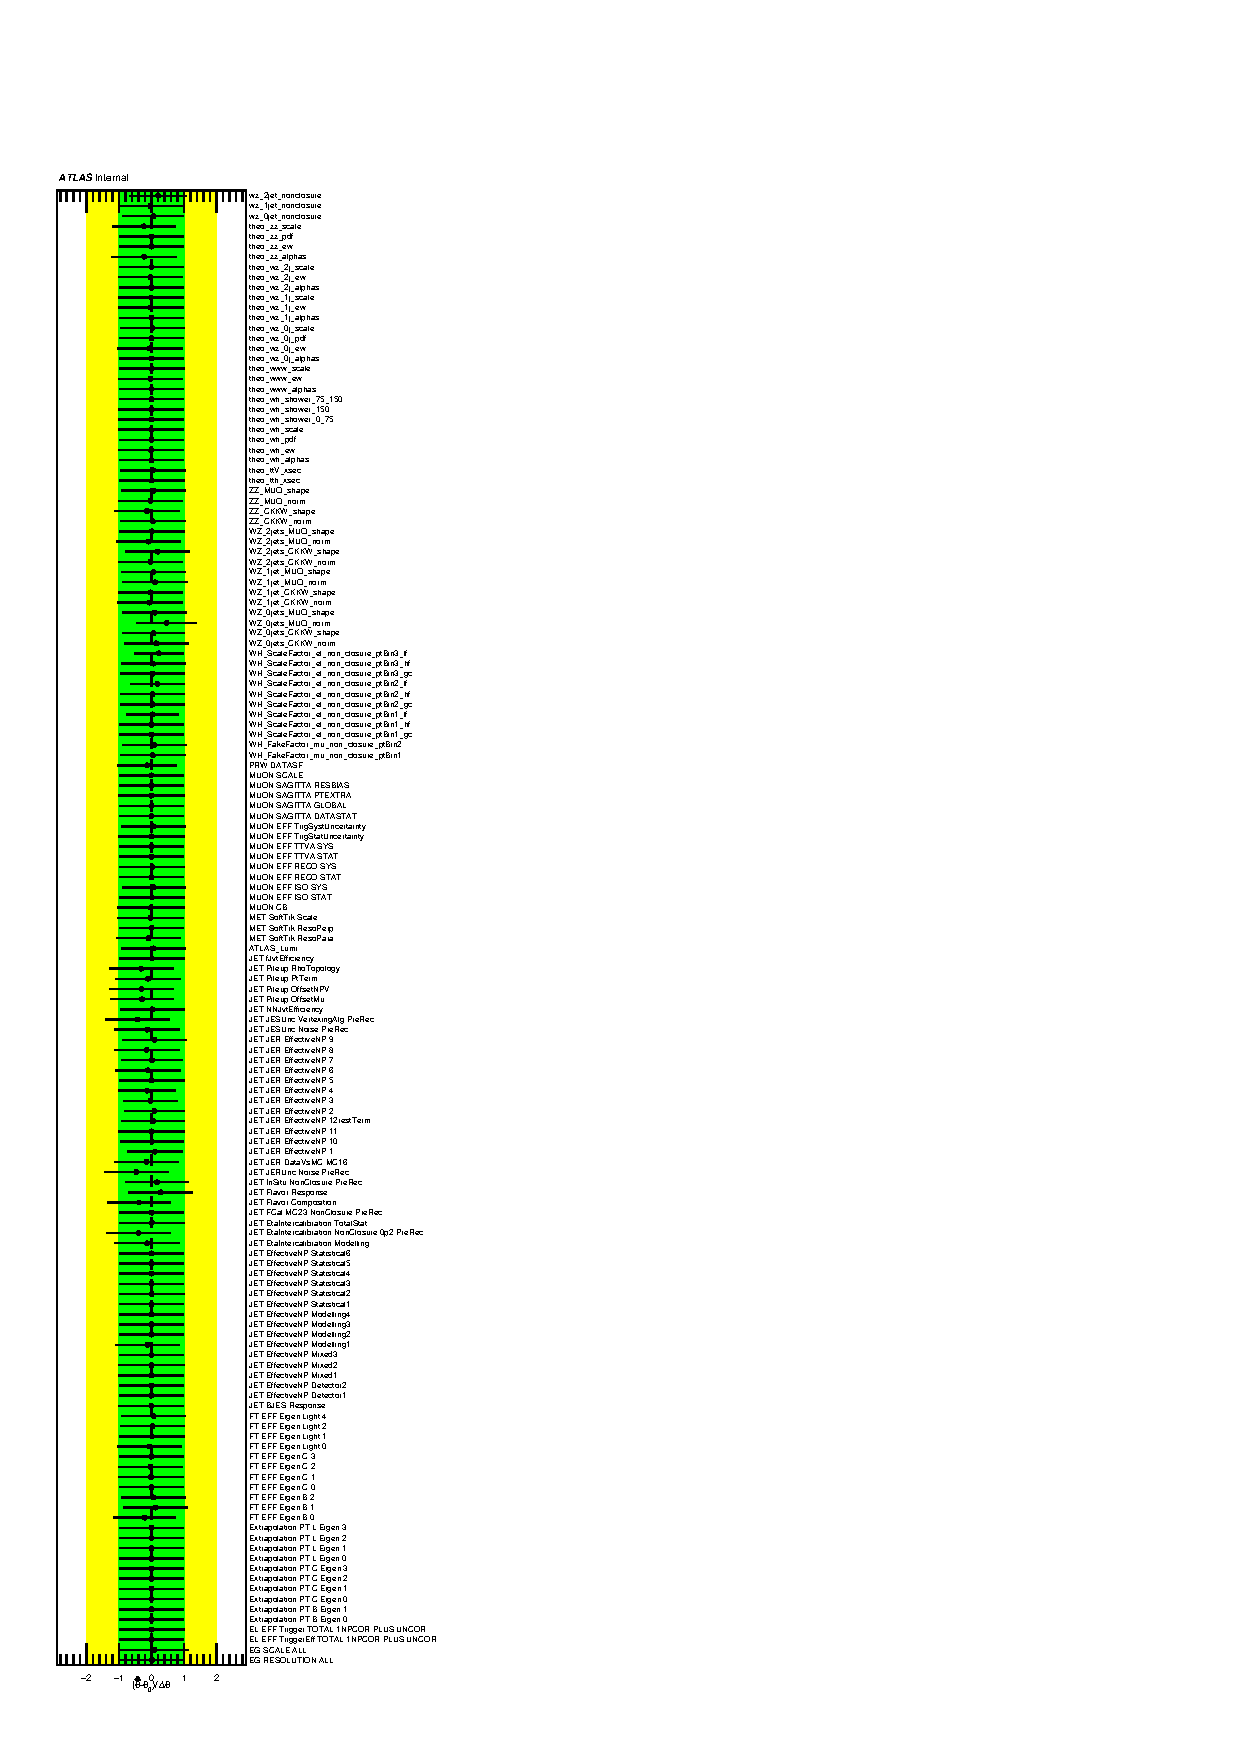
\includegraphics[width=0.33\linewidth]{figures/appendix/wh_results/pulls/NuisPar_zdom.pdf}
  }
  \subfloat[\zdep{} SR.]{
    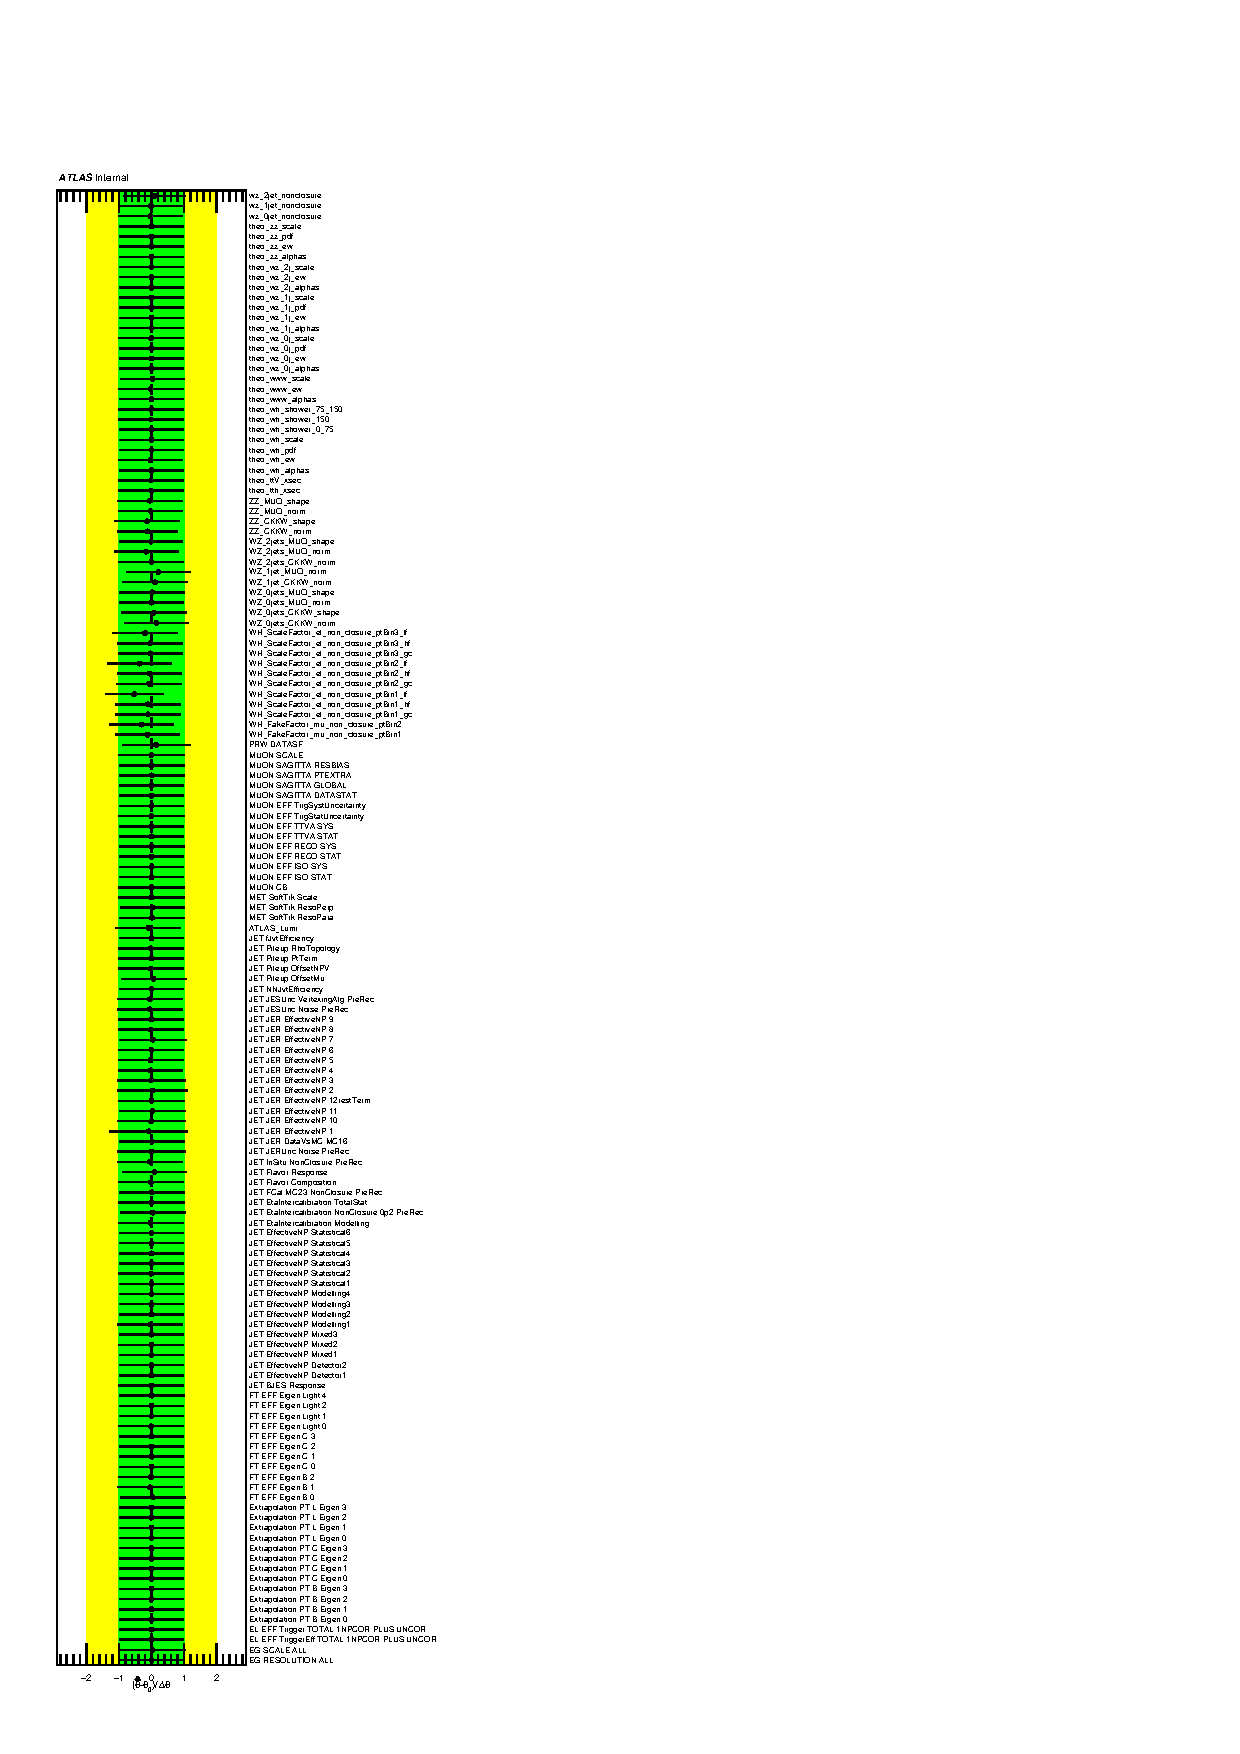
\includegraphics[width=0.33\linewidth]{figures/appendix/wh_results/pulls/NuisPar_zdep.pdf}
  }
  \subfloat[Combined \wh{} SR's.]{
    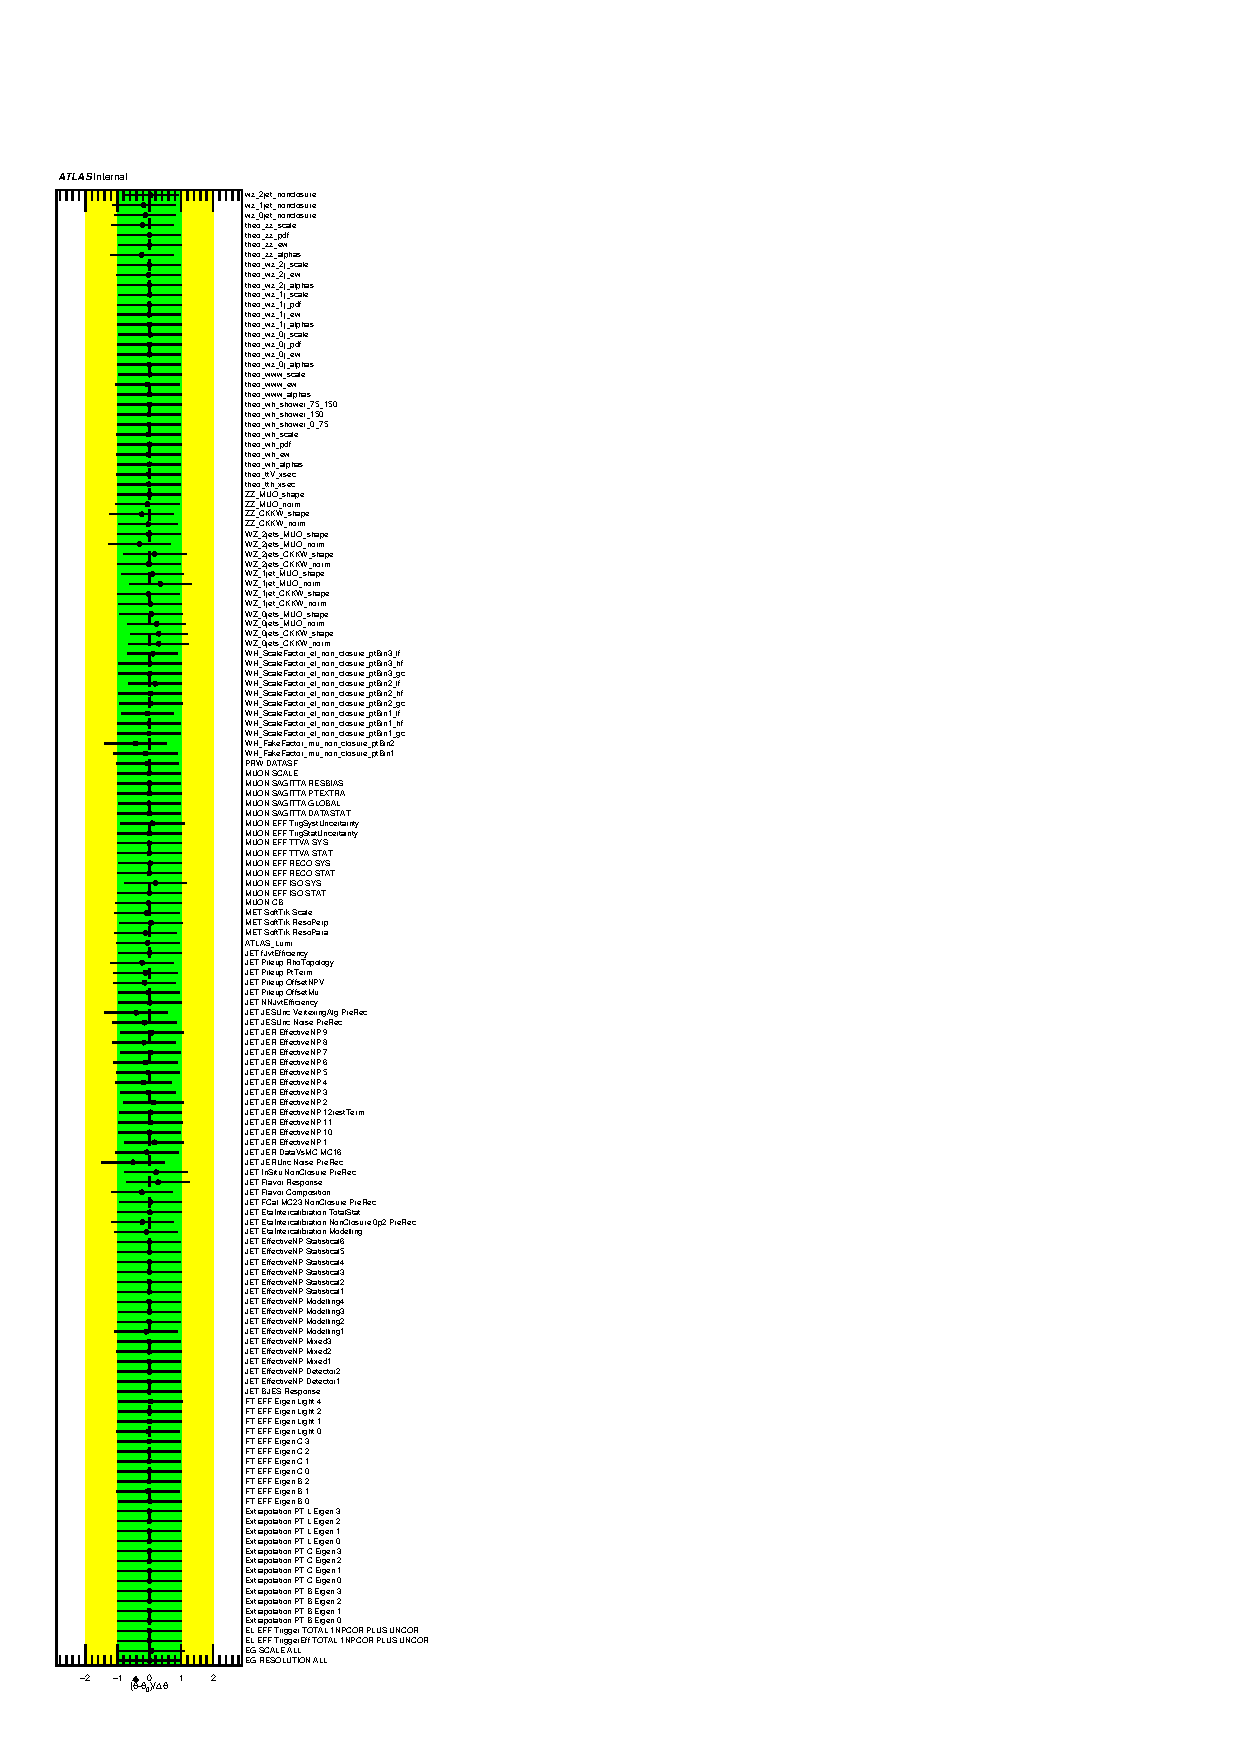
\includegraphics[width=0.33\linewidth]{figures/appendix/wh_results/pulls/NuisPar_combined.pdf}
  }
  \caption{Pull plots for the \wh{} signal regions: (a) \zdom{}, (b) \zdep{}, and (c) combined channel.}\label{fig:wh_pull_plots_zdom_zdep_expected}
\end{figure}

% \begin{figure}[htp]
%   \centering
%   \subfloat[Combined \wh{} SR's.]{
%     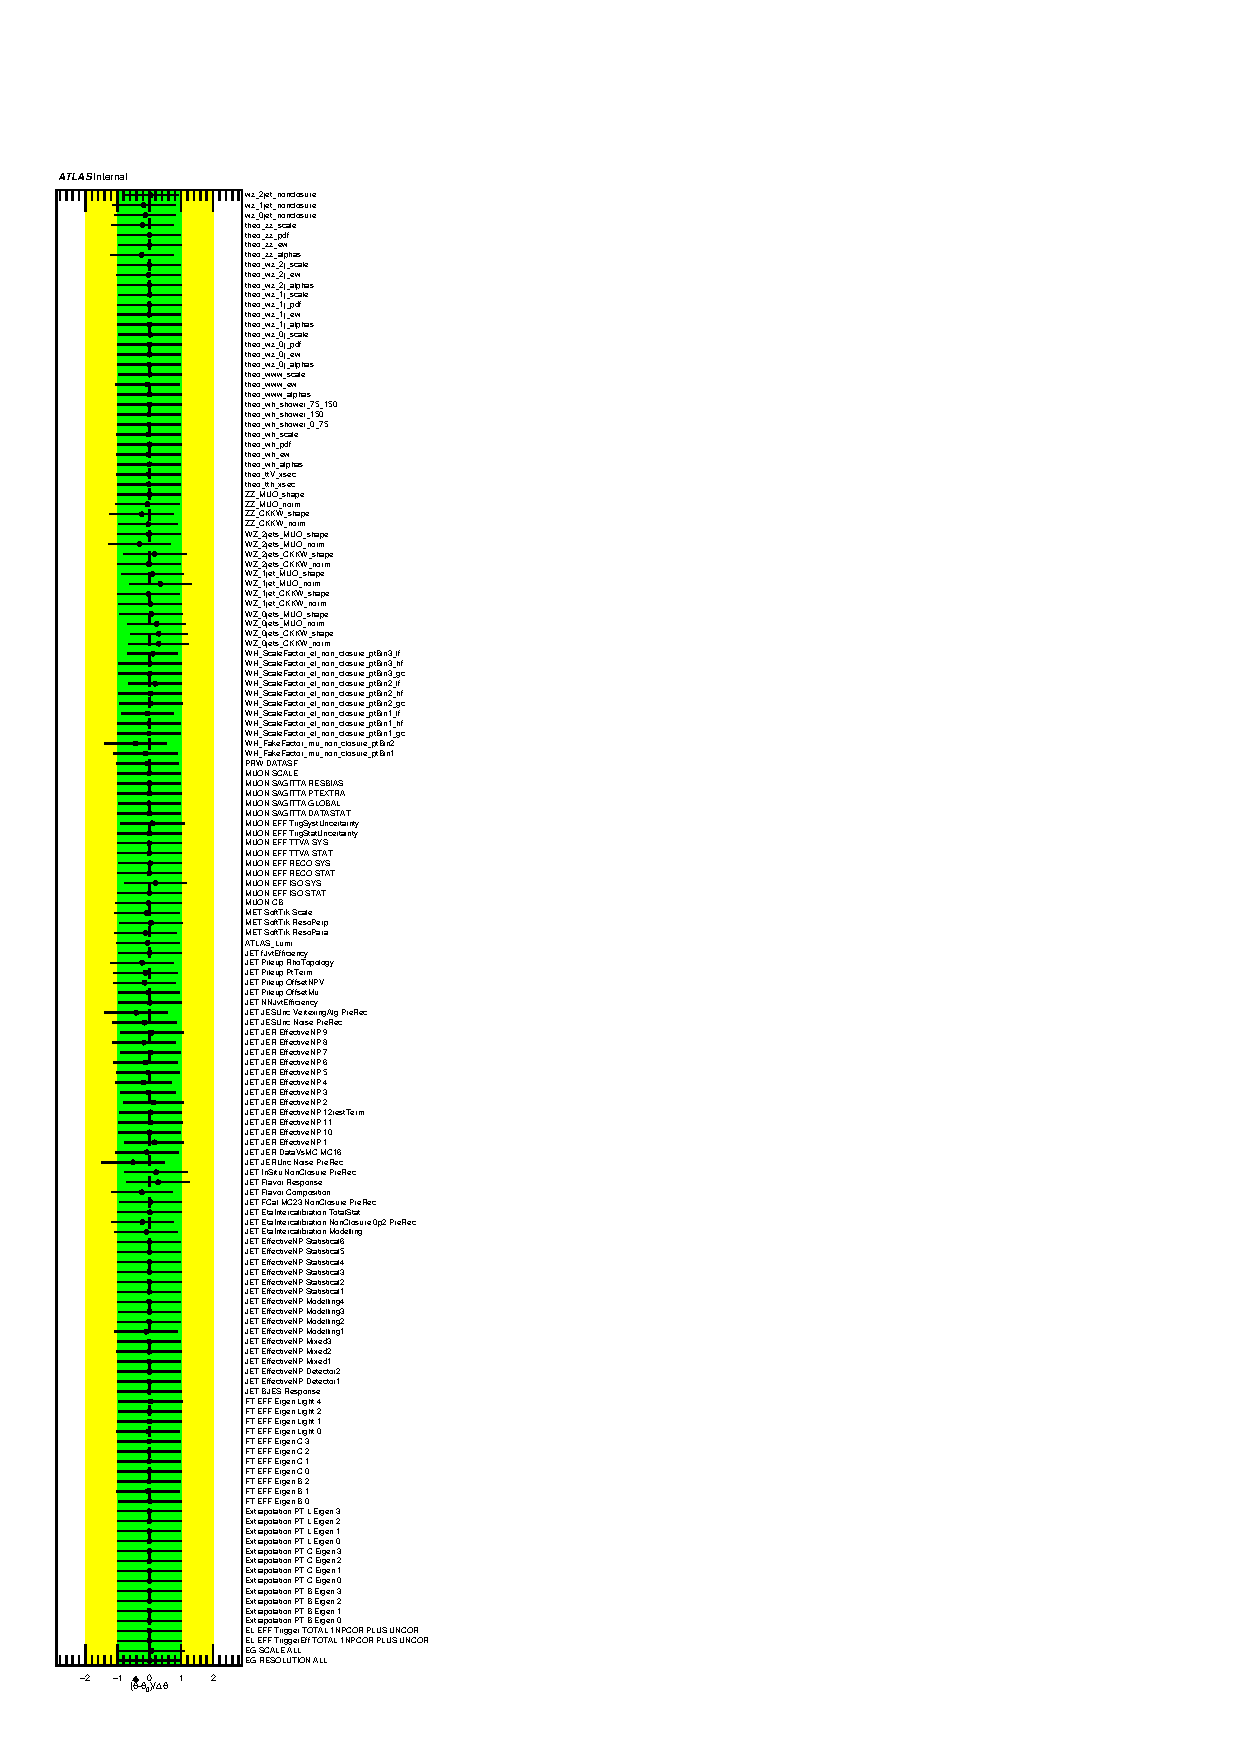
\includegraphics[width=0.33\linewidth]{figures/appendix/wh_results/pulls/NuisPar_combined.pdf}
%   }
%   \caption{Pull plot for the combined \wh{} signal regions.}\label{fig:wh_pull_plots_combined_expected}
% \end{figure}
\clearpage{}
